\let\lesson\undefined
\newcommand{\lesson}{\phantomlesson{Bài 8: Sự rơi tự do}}
\chapter[Sự rơi tự do]{Sự rơi tự do}
\setcounter{section}{0}
\section{Lý thuyết}
\subsection{Sự rơi trong không khí và sự rơi tự do}
\subsubsection{Sự rơi của các vật trong không khí}
Trong không khí sự rơi của các vật là do tác dụng bởi trọng lực và lực cản của không khí.
\subsubsection{Sự rơi tự do }
Nếu loại bỏ được ảnh hưởng của không khí thì mọi vật sẽ rơi nhanh như nhau. Sự rơi của các vật trong trường hợp này gọi là sự rơi tự do.

Sự rơi tự do là sự rơi chỉ dưới tác dụng của trọng lực.
\begin{center}
	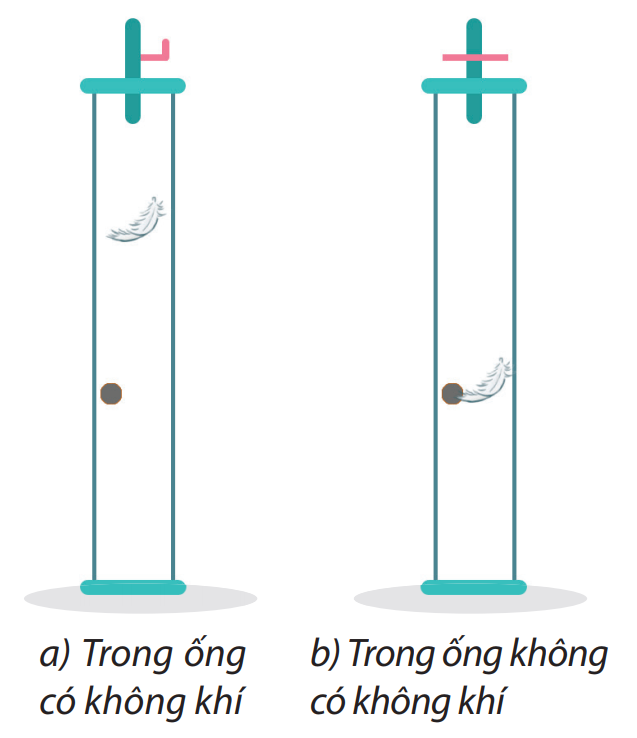
\includegraphics[width=0.25\linewidth]{../figs/VN10-2023-PH-TP011-1}
	\captionof{figure}{Thí nghiệm về sự rơi tự do.}
\end{center}
\subsection{Nghiên cứu sự rơi tự do của các vật}
\subsubsection{Những đặc điểm của chuyển động rơi tự do}
\begin{itemize}
	\item Phương của chuyển động rơi tự do là phương thẳng đứng (phương của dây dọi).
	\item Gia tốc của vật chuyển động rơi tự do chính là gia tốc rơi tự do.
	\item Chuyển động rơi tự do là chuyển động thẳng biến đổi đều.
\end{itemize}	

\subsubsection{Gia tốc rơi tự do}
Tại một nơi nhất định trên Trái Đất và ở gần mặt đất, mọi vật đều rơi tự do với cùng gia tốc.

Gia tốc rơi tự do kí hiệu là $g$, giá trị của $g$ phụ thuộc vào vĩ độ địa lí và độ cao. Ở gần bề mặt Trái Đất người ta thường lấy giá trị của $g$ bằng $\SI{9.8}{\meter/\second^2}$.
\subsubsection{Các phương trình của sự rơi tự do}

Phương trình vận tốc:

\begin{equation*}
	v = v_0+g(t -t_0).
\end{equation*}

Phương trình tọa độ (gốc toạ độ tại vị trí ban đầu của vật, chiều dương cùng chiều chuyển động):

\begin{equation*}
	y = y_0 +v_0(t-t_0)+ \dfrac{1}{2}g(t -t_0)^2.
\end{equation*}

Quãng đường đi được:

\begin{equation*}
	d= s = v_0(t-t_0)+\dfrac{1}{2} g (t-t_0)^2
\end{equation*}
Liên hệ giữa vận tốc và quãng đường đi được:
$$v^2-v^2_0=2gs$$

Nếu ta chọn $t_{0}=0$ và vật được thả rơi không vận tốc đầu $v_0=0$ thì các công thức trên trở thành
\begin{align*}
	v&=gt\\	
	y&=y_0+\dfrac{1}{2}gt^{2}\\
	d&=s=\dfrac{1}{2}gt^{2}\\
	v^2&=2gs
\end{align*}

\luuy{ 
	Định nghĩa sự rơi tự do là chuyển động chỉ dưới tác dụng của trọng lực, tức là gia tốc của vật phải đúng bằng gia tốc rơi tự do $a=g$, chứ không quy định về vận tốc ban đầu của vật. 
	
	Nói cách khác, thành phần chuyển động theo phương thẳng đứng của các vật chuyển động ném ngang, ném xiên đều được coi là chuyển động rơi tự do.
}	


\section{Mục tiêu bài học - Ví dụ minh họa}
\begin{dang}{Nhận biết được đặc điểm của sự rơi tự do, gia tốc rơi tự do}
	\viduii{1}{Câu nào sau đây nói về sự rơi là đúng?
		
		\begin{mcq}
			\item Khi không có sức cản, vật nặng rơi nhanh hơn vật nhẹ.
			\item Ở cùng một nơi, mọi vật rơi tự do có cùng gia tốc.
			\item Khi rơi tự do, vật nào ở độ cao hơn sẽ rơi với gia tốc lớn hơn.
			\item Vận tốc của vật chạm đất, không phụ thuộc vào độ cao của vật khi rơi.
		\end{mcq}
	}
	{\hide{
		Gia tốc rơi tự do $g$ không phụ thuộc khối lượng của vật, chỉ phụ thuộc vĩ độ địa lí, độ cao và cấu trúc địa chất nơi đo nó nên ở cùng một nơi, mọi vật rơi tự do có cùng gia tốc.
		
		\textbf{Đáp án: B}.
	}}
	\viduii{1}{Chuyển động của vật nào dưới đây có thể coi gần đúng như chuyển động rơi tự do?
		\begin{mcq}(2)
			\item Một vận động viên nhảy dù đang rơi khi dù đã mở. 
			\item Một viên gạch rơi từ độ cao $\SI{3}{m}$ xuống đất.
			\item Một chiếc thang máy đang chuyển động đi xuống.  
			\item Một chiếc lá đang rơi. 
		\end{mcq}
	}
	{\hide{
		Theo định nghĩa, sự rơi tự do (chuyển động rơi tự do) là sự rơi của các vật chỉ chịu tác dụng của trọng lực.
		
		Trong các trường hợp trên, vận động viên nhảy dù và chiếc lá đều chịu thêm tác động của lực cản không khí trong quá trình rơi; thang máy chịu thêm tác động của lực căng dây cáp. Các lực thêm vào này làm chuyển động của các vật này có gia tốc khác đáng kể với gia tốc rơi tự do. Do đó, các  chuyển động này không được xem là chuyển động rơi tự do. 
		
		Chuyển động của một viên gạch rơi từ độ cao $\SI{3}{m}$ xuống đất có thể xem gần đúng là chuyển động rơi tự do, vì trong khi rơi lực cản không khí không đáng kể so với trọng lực, nên gia tốc của viên gạch gần bằng gia tốc rơi tự do.
		
		\textbf{Đáp án: B}.
	}}
	
	\viduii{1}{Chọn phương án sai. Chuyển động rơi tự do không vận tốc đầu có
		\begin{mcq}(2)
			\item phương thẳng đứng.
			\item chiều từ trên xuống dưới.
			\item là chuyển động thẳng chậm dần đều.
			\item chỉ chịu tác dụng của trọng lực. 
		\end{mcq}
	}
	{\hide{
		Chuyển động rơi tự do không vận tốc đầu là chuyển động thẳng nhanh dần đều.
		
		\textbf{Đáp án: C}.
	}}
	
\end{dang}
%\begin{dang}{Ghi nhớ được hệ quả \\từ thí nghiệm của Niutơn}
%	\viduii{1}{Vật nào được xem là rơi tự do?
	%		\begin{mcq}
		%			\item Viên đạn đang bay trên không trung.
		%			\item Phi công đang nhảy dù (đã bật dù).
		%			\item Quả táo đang rơi từ trên cây xuống.
		%			\item Máy bay đang bay.
		%		\end{mcq}
	%	}
%	{	\begin{center}
		%			\textbf{Hướng dẫn giải}
		%		\end{center}
	
	%		Dựa vào khái niệm sự rơi tự do: "Sự rơi tự do là sự rơi chỉ dưới tác dụng của trọng lực".
	
	%		Quả táo đang rơi thỏa mãn điều kiện của sự rơi tự do.
	
	%		\textbf{Đáp án: C}.
	%	}

%	\viduii{1}{Chuyển động của vật nào dưới đây có thể coi như chuyển động rơi tự do?
	%		\begin{mcq}
		%			\item Một vận động viên nhảy dù đang rơi khi dù đã mở. 
		%			\item Một viên gạch rơi từ độ cao $\SI{3}{m}$ xuống đất.
		%			\item Một chiếc thang máy đang chuyển động đi xuống.  
		%			\item Một chiếc lá đang rơi. 
		%		\end{mcq}
	%	}
%	{	\begin{center}
		%			\textbf{Hướng dẫn giải}
		%		\end{center}
	
	%		Ta có: Sự rơi tự do (chuyển động rơi tự do) là sự rơi của các vật chỉ chịu tác dụng của trọng lực.
	
	%		Chuyển động của một viên gạch rơi từ độ cao $\SI{3}{m}$ xuống đất là chuyển động rơi tự do.
	
	%		\textbf{Đáp án: B}.
	%	}


%\end{dang}
% Hưng's comment: nội dung mục này không khác mục trước, cũng không rõ thí nghiệm của Newton là thí nghiệm nào (trong bài học không nhắc đến) nên tiêu đề không rõ ràng. 
%\begin{dang}{Nhận biết được công thức xác định \\ vận tốc, quãng đường và thời gian rơi tự do}
%	\viduii{1}{Chọn phát biểu sai về chuyển động rơi tự do.
%		\begin{mcq}
%			\item Vật có khối lượng càng lớn rơi càng nhanh.
%			\item Đại lượng đặc trưng cho sự biến thiên vận tốc là gia tốc trọng trường.
%			\item Vật có vận tốc cực đại khi chạm đất.
%			\item Sự rơi tự do là sự rơi chỉ chịu tác dụng của trọng lực.
%		\end{mcq}
%	}
%	{	\begin{center}
%			\textbf{Hướng dẫn giải}
%		\end{center}
%		
%		Thời gian rơi tự do được xác định từ các phương trình chuyển động. Các phương trình này không phụ thuộc vào khối lượng, do đó nhận định ở đáp án A không đúng. 
%		
%		
%		\textbf{Đáp án: A}.
%	}
%	\viduii{1}{Chọn câu sai
%		\begin{mcq}
%			\item Vật rơi tự do khi không chịu sức cản của môi trường.
%			\item Khi rơi tự do các vật chuyển động giống nhau.
%			\item Công thức $s =\dfrac{1}{2} gt^2$ dùng để xác định quãng đường đi được của vật rơi tự do không vận tốc đầu.
%			\item Có thể coi sự rơi của chiếc lá khô từ trên cây xuống là sự rơi tự do.
%		\end{mcq}
%	}
%	{	\begin{center}
%			\textbf{Hướng dẫn giải}
%		\end{center}
%		
%		Sự rơi tự do là sự rơi chỉ chịu tác dụng của trọng lực, còn chiếc lá khô rơi từ trên cây xuống còn chịu thêm lực cản của không khí.
%		
%		\textbf{Đáp án: D}.
%	}
%	
%\end{dang}
% Sang: Phần này chỉ là các câu hỏi lý thuyết, ko rõ được mục tiêu nhận biết phương trình ... ở điểm nào.
\begin{dang}{Xác định vận tốc, quãng đường và thời gian của vật rơi tự do}
	
	\viduii{2}{Một vật rơi tự do không vận tốc đầu, khi chạm đất thì vật đạt tốc độ $v = \SI{20}{m/s}$. Hỏi vật được thả rơi từ độ cao nào? Biết $g = \SI{10}{m/s}^2$.
	}
	{\hide{
	Ta có:
	$$v^2-v^2_0=2gh\Rightarrow h=\dfrac{v^2}{2g}=\dfrac{\left(\SI{20}{\meter/\second}\right)^2}{2\cdot\left(\SI{10}{\meter/\second^2}\right)}=\SI{20}{\meter}.$$
	
	}}
	\viduii{2}{
		Từ độ cao $\SI{120}{m}$ người ta thả một vật thẳng đứng xuống với vận tốc đầu $v_0 = \SI{10}{m/s}$. Cho biết gia tốc trọng trường $g = \SI{10}{m/s}^2$.
		\begin{enumerate}[label=\alph*.]
			\item Sau bao lâu vật chạm đất.
			\item Tính vận tốc của vật lúc vừa chạm đất. 
		\end{enumerate}
	}
	{\hide{
		\begin{enumerate}[label=\alph*.]
			\item Thời gian vật chạm đất được tính từ phương trình chuyển động
			
			$$s = v_0t + \dfrac{1}{2}gt^2 \quad\Leftrightarrow\quad 120 = 10t + 5t^2.$$
			Giải phương trình này, ta thu được hai nghiệm và chọn nghiệm dương
			$$\Rightarrow t = \SI{4}{s}\ (\text{nhận})\ \text{hoặc} \ t = -\SI{6}{s}\ (\text{loại}).$$
			
			\item Vận tốc của vật lúc vừa chạm đất
			$$v = v_0 + gt =\SI{10}{\meter/\second}+(\SI{10}{\meter/\second^{2}})\times\left(\SI{4}{\second}\right)= \SI{50}{m/s}.$$
		\end{enumerate}	
		\luuy{Trong khi giải các phương trình chuyển động thẳng biến đổi đều để tìm thời gian, ta thường gặp trường hợp giải được hai nghiệm. Thông thường nghiệm dương sẽ được chọn vì đây là nghiệm ứng với thời điểm sau khi bắt đầu khảo sát hiện tượng.  }		
	}}
\end{dang}
\begin{dang}{Lập phương trình chuyển động của vật rơi tự do}
	\viduii{3}{Từ một đỉnh tháp cao $\SI{20}{\meter}$, người ta buông một vật. Sau $\SI{2}{\second}$ thì người ta lại buông vật thứ 2 ở tầng thấp hơn đỉnh tháp $\SI{5}{\meter}$. Chọn trục O$y$ thẳng đứng, gốc O ở đỉnh tháp, chiều dương hướng xuống, mốc thời gian lúc vật 1 bắt đầu rơi, $g=\SI{10}{\meter/\second^2}$.
		\begin{enumerate}[label=\alph*.]
			\item Lập phương trình chuyển động của hai vật.
			\item Hai vật có chạm đất cùng lúc không?
			\item Vận tốc lúc chạm đất của mỗi vật là bao nhiêu?
		\end{enumerate}
	}
	{\hide{
		\begin{enumerate}[label=\alph*.]
			\item 
			Vật thứ nhất xuất phát từ đỉnh tháp (là gốc tọa độ) và được buông (không vận tốc đầu) nên phương trình chuyển động có dạng 
			\begin{align*}
				y_1&=y_{01}+v_{01}t+\dfrac{1}{2}gt^2\\
				&=\SI{0}{\meter}+ \left(\SI{0}{\meter/\second}\right)\times t +\dfrac{1}{2}\times\left(\SI{10}{\meter/\second^{2}}\right)\times t^{2}\\
				&=5t^{2} \quad \left(\si{\meter}, \si{\second}\right).
			\end{align*}
			
			Phương trình chuyển động của vật 2 là:
			\begin{align*}
				y_{2}&=y_{02}+v_{02}t+\dfrac{1}{2}g(t-t_0)^2\\
				&=\SI{5}{\meter}+(\SI{0}{\meter/\second})\times (t-\SI{2}{\second})+\dfrac{1}{2}\times(\SI{10}{\meter/\second^{2}})\times (t-\SI{2}{\second})^{2}\\
				&=5t^2-20t+25\quad \left(\si{\meter}, \si{\second}\right)\qquad \textrm{với }t>2.
			\end{align*}
			\item 
			Thời điểm vật 1 chạm đất:
			\begin{equation*}
				y_1=5t^2=\SI{20}{\meter}\Rightarrow t_1=\SI{2}{\second}.
			\end{equation*}
			
			Thời điểm vật 2 chạm đất:
			\begin{equation*}
				\begin{gathered}
					y_{2}=5t^2-20t+25=\SI{20}{\meter}\\ \quad\Rightarrow\quad t_2=\SI{3.73}{\second}\textrm{ (nhận) hoặc } t_2=\SI{0.27}{\second}\textrm{ (loại)}.
				\end{gathered}
			\end{equation*}
			Ở đây nghiệm $\SI{0.27}{\second}$ bị loại vì đây là thời điểm trước khi vật 2 được thả, không phù hợp với hiện tượng được mô tả trong đề. 
			
			Vậy hai vật không chạm đất cùng lúc.
			\item Vận tốc lúc chạm đất của mỗi vật là:
			\begin{align*}
				v_1&=gt_1=\left(\SI{10}{\meter/\second^{2}}\right)\times\left(\SI{2}{\second}\right)=\SI{20}{\meter/\second},\\
				v_2&=g(t_2-t_0)=\left(\SI{10}{\meter/\second^{2}}\right)\times(\SI{3.73}{\second}-\SI{2}{\second})=\SI{17.3}{\meter/\second}.
			\end{align*}
		\end{enumerate}
	}}
	
\end{dang}

\begin{dang}{Xác định quãng đường vật đi được \\trong giây thứ $n$, hoặc trong $n$ giây cuối}
	\ppgiai{
		Quãng đường rơi được trong $n$ giây kể từ thời điểm được thả rơi: 
		$$s_n=\dfrac{1}{2}\cdot g \cdot n^2$$
		Quãng đường rơi được trong giây thứ $n$ là quãng đường vật đi được từ thời điểm $\left(n-1\right)$ giây đến thời điểm $n$ giây
		$$\Delta s_n=s_n-s_{n-1}=\dfrac{1}{2}\cdot g\cdot n^2 -\dfrac{1}{2}\cdot g \left(n-1\right)^2$$
	}
\viduii{3}{Một vật rơi tự do không vận tốc đầu tại nơi có gia tốc trọng trường $g$. Trong giây thứ 3, quãng đường rơi được là $\SI{24,5}{m}$ và tốc độ của vật khi vừa chạm đất là $\SI{39,2}{m/s}$. Tính gia tốc trọng trường $g$ tại nơi thả vật và độ cao ban đầu của vật.
}
{\hide{
	Quãng đường vật rơi trong 3 giây: 
	$$s_1 = \dfrac{1}{2}gt^2_1 =\text{4,5}g.$$	
	
	Quãng đường vật rơi trong 2 giây đầu: 
	$$s_2 = \dfrac{1}{2}gt^2_2 =2g.$$	
	
	Quãng đường vật rơi trong giây thứ 3: 
	$$\Delta s = s_1 - s_2 \quad\Leftrightarrow\quad \text{24,5} = \text{4,5}g - 2g \quad\Rightarrow g = \SI{9,8}{m/s}^2.$$

	Độ cao lúc thả vật: 
	$$s =\dfrac{v^2}{2g} =\SI{80}{m}.$$
	
}}
	\viduii{3}{Một vật rơi tự do từ độ cao $h$. Biết rằng trong $\SI{2}{s}$ cuối cùng vật rơi được quãng đường bằng quãng đường đi trong $\SI{5}{s}$ đầu tiên, $g = \SI{10}{m/s}^2$.
		\begin{enumerate}[label=\alph*.]
			\item Tìm độ cao lúc thả vật và thời gian vật rơi.
			
			\item Tìm tốc độ của vật lúc vừa chạm đất.
			
		\end{enumerate}
	}
	{\hide{
		\begin{enumerate}[label=\alph*.]
			\item Chọn chiều dương hướng xuống, gốc toạ độ tại vị trí vật bắt đầu rơi, gốc thời gian lúc vật rơi. 
			
			Quãng đường vật rơi trong $t$ giây: 
			$$s = \dfrac{1}{2}gt^2.$$
			
			Quãng đường vật rơi trong ($t - 2$) giây: 
			$$s_1 =\dfrac{1}{2}g(t-2)^2.$$
			
			Quãng đường vật rơi trong 5 giây đầu tiên: 
			$$s_5 = \dfrac{1}{2}gt_5^2.$$
			
			Quãng đường vật rơi trong 2 giây cuối: 
			$$s_2 = s - s_1 = s_5 \quad\Leftrightarrow\quad  \dfrac{1}{2}gt^2 - \dfrac{1}{2}g(t-2)^2 = \dfrac{1}{2}gt_5^2 \quad\Rightarrow\quad t = \SI{7,25}{s}.$$
			
			Độ cao lúc thả vật:
			$$s = \dfrac{1}{2}gt^2= \SI{262,81}{m}.$$
			\item  Tốc độ của vật lúc vừa chạm đất:
			
			$$v = gt = \SI{72,5}{m/s}.$$
		\end{enumerate}
	}}
	
\end{dang}
\begin{dang}{Khảo sát chuyển động của vật bị ném theo phương thẳng đứng}
		\viduii{2}{Một vật được ném lên thẳng đứng từ mặt đất, bỏ qua lực cản của không khí. Tính độ cao cực đại mà vật đạt được biết vận tốc ban đầu của vật là $\SI{20}{m/s}$, lấy $g = \SI{10}{m/s^2}$.
	}
	{\hide{
		Chọn chiều dương hướng lên, chuyển động của vật là chuyển động thẳng chậm dần đều với gia tốc $a = -g = -\SI{10}{m/s^2}$ và vận tốc ban đầu $v_0=\SI{20}{m/s}.$
		
		Độ cao cực đại bằng quãng đường mà vật đi được đến khi dừng lại ($v=0$)
		$$v^2 - v_0^2=2as \Rightarrow s= h_\text{max}= \SI{20}{m}.$$
	}}

	\viduii{3}{Một vật được ném lên theo phương thẳng đứng từ mặt đất. Sau $\SI{4}{s}$ vật lại rơi xuống mặt đất. cho $g = \SI{10}{m/s}^2$. Tính
		\begin{enumerate}[label=\alph*)]
			\item Vận tốc ban đầu của vật.
			
			\item Độ cao tối đa mà vật lên tới
			
			\item Vận tốc của vật ở độ cao bằng $\dfrac{3}{4}$ độ cao tối đa.
		\end{enumerate}
	}
	{\hide{
		\begin{enumerate}[label=\alph*)]
			\item Chọn gốc toạ độ tại vị trí ném, chiều dương hướng lên, gốc thời gian lúc ném vật. Phương trình chuyển động của vật có dạng 
			$$y =v_0t - \dfrac{1}{2}gt^2.$$
			Vật chạm đất khi $y=0$, do đó 
			\begin{align*}
				y&= v_0t -\dfrac{1}{2}gt^2=0\\
				\Rightarrow\quad v_0 &=\dfrac{gt}{2}=\dfrac{
					\SI{10}{\meter/\second^2}\cdot
					\SI{4}{\second}
				}{2} =\SI{20}{\meter/\second}.
			\end{align*}
			\item Khi vật lên đến độ cao tối đa, vận tốc của vật triệt tiêu $v=0$. Độ cao của vật khi đó cũng chính là quãng đường vật đã đi được 
			\begin{align}
				v^2-v_0^2 =-2gh \quad\Rightarrow\quad h =\dfrac{v^2 -v_0^2}{-2g}=\dfrac{(\SI{0}{\meter/\second})^2-(\SI{20}{\meter/\second})^2}{-2\cdot\SI{10}{\meter/\second^{2}}}=\SI{20}{\meter}.
			\end{align}
			\item Sử dụng công thức liên hệ 
			$v_1^2-v_0^2 =2as=-2gh_1,$ 
			trong đó độ cao $h_1=\dfrac{3}{4}h=\SI{15}{m}$,
			ta suy ra vận tốc của vật khi đó 
			\begin{eqnarray*}
				v_1^2&=&v_0^2 -2gh_1=(\SI{20}{\meter/\second})^2-2\cdot\SI{10}{\meter/\second^{2}}\cdot\SI{15}{\meter}=\SI{100}{\meter^2/\second^2}\\
				\Rightarrow\quad v_1&=&\pm \SI{10}{\meter/\second}.
			\end{eqnarray*}
			Giá trị dương của vận tốc ứng với thời điểm vật đang đi lên, giá trị âm ứng với thời điểm vật đang đi xuống. 
		\end{enumerate}
	}}

	\viduii{3}{
	Một viên bi A được thả rơi từ độ cao $\SI{30}{\meter}$. Cùng lúc đó, một viên bi B được bắn theo phương thẳng đứng từ dưới đất lên với vận tốc ban đầu $\SI{25}{\meter/\second}$ tới va chạm vào bi A. Chọn trục O$y$ thẳng đứng, gốc O ở mặt đất, chiều dương hướng lên, gốc thời gian lúc 2 viên bi bắt đầu chuyển động, $g=\SI{10}{\meter/\second^2}$. Bỏ qua sức cản không khí.
	\begin{enumerate}[label=\alph*.]
		\item Lập phương trình chuyển động của mỗi viên bi.
		\item Tính thời điểm và tọa độ 2 viên bi gặp nhau.
		\item  Vận tốc mỗi viên bi khi gặp nhau.
	\end{enumerate}
}
{\hide{
	\begin{enumerate}[label=\alph*.]
		\item 
		Phương trình chuyển động của viên bi A là
		\begin{align*}
			y_{\text{A}}&=y_{0\text{A}}+v_{0\text{A}}t+\dfrac{1}{2}gt^2\\
			&=30+0\times t-\dfrac{1}{2}\times 10\times t^{2}\\
			&=30-5t^2 \textrm{ (m, s)}.
		\end{align*}
		
		Phương trình chuyển động của viên bi B là
		\begin{align*}
			y_{\text{B}}&=y_{0\text{B}}+v_{0\text{B}}t+\dfrac{1}{2}gt^2\\
			&=0+25t-\dfrac{1}{2}\times10\times t^{2}\\
			&=25t-5t^2\textrm{ (m, s)}.
		\end{align*}
		\item 
		Hai viên bi gặp nhau khi chúng có cùng tọa độ
		\begin{equation*}
			y_{\text{A}}=y_{\text{B}}\Rightarrow 30-5t^2=25t-5t^2 \Rightarrow t=\SI{1.2}{\second}.
		\end{equation*}
		
		Khi đó hai viên bi đang ở tọa độ 
		\begin{equation*}
			y_{\text{A}}=y_{\text{B}}=30-5t^2=\SI{22.8}{\meter}.
		\end{equation*}
		\item  Vận tốc của mỗi viên bi khi gặp nhau là:
		\begin{equation*}
			\left\{\begin{array}{ll}{v_{\text{A}}=-gt=\SI{-12}{\meter/\second}}&\\{v_{\text{B}}=v_0-gt=\SI{13}{\meter/\second}.}&\end{array}\right.
		\end{equation*}
		Vận tốc của bi 1 âm cho thấy bi 1 đang chuyển động hướng xuống (ngược chiều dương), còn bi 2 có vận tốc dương cho tương ứng đang chuyển động hướng lên (cùng chiều dương).
	\end{enumerate}
}}

\end{dang}

